\documentclass{article}
\usepackage[a4paper]{geometry}
\usepackage[italian]{babel}
\usepackage[parfill]{parskip}
\usepackage[utf8]{inputenc}
\usepackage{amsfonts} 
\usepackage{amsmath}
\usepackage{enumitem}
\usepackage{graphicx}
\usepackage{hyperref}
\usepackage{listings}
\usepackage{natbib}
\usepackage{xcolor}

% modulo
\newcommand{\Mod}[1]{\ (\mathrm{mod}\ #1)}
% insiemi
\newcommand{\Kp}{\mathbb{K}_{p}}
\newcommand{\Zp}{\mathbb{Z}_{p}}

\definecolor{codegreen}{HTML}{1E5E19}
\definecolor{codegray}{HTML}{1E5E19}
\definecolor{codepurple}{HTML}{1E5E19}
\definecolor{backcolour}{HTML}{FAFAFA}

\lstdefinestyle{mystyle}{
    backgroundcolor=\color{backcolour},   
    commentstyle=\color{codegreen},
    keywordstyle=\color{magenta},
    numberstyle=\tiny\color{codegray},
    stringstyle=\color{codepurple},
    basicstyle=\ttfamily\footnotesize,
    breakatwhitespace=false,         
    breaklines=true,                 
    captionpos=b,                    
    keepspaces=true,                 
    numbers=left,                    
    numbersep=5pt,                  
    showspaces=false,                
    showstringspaces=false,
    showtabs=false,                  
    tabsize=2
}

\title{Matematica, codice e crittografia in Bitcoin}

\author{Luca Polverini \\ email luca.polverini@gmail.com}

\date{2020}

\usepackage{natbib}
\usepackage{graphicx}

\begin{document}

\maketitle

% \twocolumn

\newpage

\tableofcontents

\newpage

\part{Bitcoin}

\section{Introduzione}

\textbf{Bitcoin} è una valuta digitale \textit{sperimentale} che consente pagamenti istantanei senza confini (\textit{border-less})
verso "chiunque" nel mondo e senza ricorso ad una autorità centrale (la banca).

Nel corso della storia moderna sono stati effettuati vari tentativi di creare una valuta digitale, per lo più fallimentari.

Nel 2008, Satoshi Nakamoto \footnote{(uno pseudonimo dietro al quale si cela un lui, un lei, un gruppo di persone o una associazione)} 
pubblica un \textit{white-paper}\cite{Nakamoto} mettendo in luce un metodo per risolvere il problema della doppia spesa (\textit{double-spending})
in un contesto decentralizzato, senza ricorrere alla "zecca", dando così vita alla tecnologia \textit{block-chain} in generale e alle cripto-valute in particolare.

Le caratteristiche fondanti della tecnologia blockchain sono essenzialmente tre:

\begin{itemize}
    \item architettura distribuita \textit{peer-to-peer}
    \item ricorso alla \textit{crittografia} (hashing e firma digitale)
    \item risoluzione del \textit{Problema del Generale Bizantino} (\textit{double-spending}) attraverso meccanismi di consenso (\textit{Proof of Work} in Bitcoin)
\end{itemize}

\subsection{Architettura punto a punto}

L'architettura punto-a-punto consente di distribuire il libro mastro (\textit{ledger}) delle transazioni su tutti i nodi della rete,
indipendentemente da una organizzazione centrale. Per fare un parallelo, quando visitiamo un sito web richiediamo e riceviamo
contenuti da "un server centrale" (ad esempio Facebook o Google); nel caso punto-a-punto non esiste un server centrale
ma una collezione di nodi indipendenti che replicano i contenuti e che possono fornirli su richiesta.
Ne consegue che i contenuti non sono gestiti da un unico soggetto  ma sono custoditi, gestiti e resi disponibili da molti soggetti fra loro indipendenti.

\subsection{Crittografia}

\subsubsection{Hash}

La funzione di \textit{hash} consente di associare dati di arbitraria lunghezza a codici univoci di lunghezza definita (e.g. 256 bit).
Possiamo pensare all'hash come una mappa unidirezionale che a partire da un contenuto ne deriva in maniera deterministica un indice univoco di lunghezza finita.
Il contenuto prende il nome di pre-immagine e l'hash prende il nome di immagine. Ad ogni pre-immagine corrisponde una ed una sola immagine (ai fini pratici).
L'algoritmo di hasing è veloce ma non è computazionalmente possibile la ricostruzione della pre-immagine a partire dal codice hash e la probabilità che due
contenuti diano luogo allo stesso hash, utilizzando algoritmi sicuri (tipo shasum-256) è praticamente irrilevante.
Inoltre, piccole variazioni del contenuto danno luogo a hash molto differenti.
Questo permette di referenziare utenti, transazioni e blocchi per mezzo di codici crittograficamente sicuri.

Ricapitolando, dato un messaggio, idealmente il suo hash:

\begin{itemize}
    \item è univoco e deterministico dato un messaggio esiste uno ed un solo hash (in pratica)
    \item è unidirezionale, altamente improbabile risalire al messaggio originale
    \item è veloce da computare
\end{itemize}

\subsubsection{Firma digitale}

La firma digitale (correntemente ECDSA in Bitcoin) consente di:

\begin{itemize}
    \item dimostrare la proprietà di moneta (UTXO) attraverso la coppia chiave pubblica e privata
    \item firmare il trasferimento di moneta verso un secondo soggetto attraverso l'impiego della chiave privata
    \item consentire ai nodi partecipanti della rete la verifica della liceità delle operazioni
\end{itemize}

\subsection{Consenso}

Il meccanismo di consenso permette ai nodi di concordare l'estensione del libro mastro inserendo nuove transazioni nella block-chain.

Le transazioni \textbf{valide} inviate dagli utenti vengono propagate dai nodi a tutta la rete. I nodi di tipo \textit{miner} (minatori), come vedremo nel seguito, raccolgono le transazioni e competono per
costruire un nuovo blocco che le contenga da aggiungere alla catena. 

Ne deriva che ogni neo-blocco è una entità che contiene le transazioni che vi sono state inserite dal nodo miner che è riuscito per primo a crearlo. 
Per essere aggiunto alla catena il blocco deve possedere i requisiti di validità previsti dal protocollo e deve essere validato da tutti i nodi della rete
attraverso un \textbf{meccanismo di consenso}.

Il meccanismo di consenso di Bitcoin prende il nome di \textit{Proof of Work}.
Per brevità, nel seguito, ci riferiremo alla \textit{Proof of Work} con l'acronimo \textbf{PoW}.

L'algoritmo PoW è progettato in modo tale da rendere altamente improbabile la modifica fraudolenta della catena se non possedendo almeno il 51\% delle risorse hardware dell'intera rete (una cpu, un voto \cite{Nakamoto})\footnote{in ottica evolutiva, nel seguito, esamineremo alcune non linearità}; 

PoW è difficile, non complicato; si tratta di un algoritmo semplice (computazione di codici hash) ma ad ogni tentativo di "soluzione" corrisponde una probabilità di successo molto bassa (modulata programmaticamente dal protocollo per produrre circa 2016 blocchi ogni due settimane) risultando di fatto molto dispendioso in termini di tempo, 
risorse hardware ed energetiche e fa parte degli stratagemmi progettuali atti a garantire la sicurezza della catena in un contesto distribuito.

Se da un lato la "difficoltà" della PoW serve per proteggere l'integrità della catena (libro mastro o \textit{ledger}) richiedendo risorse hardware consistenti,
dall'altro consente ai nodi minatori di essere remunerati per la loro attività. La creazione di un nuovo blocco remunera il nodo miner attraverso un sussidio e le commissioni associate alle transazioni. 

Si può affermare che Bitcoin faccia sapiente uso della teoria dei giochi \footnote{sempre in ottica evolutiva, esistono critiche circa le tendenze centralizzatrici} per garantire sicurezza ed equilibrio nel quadro di un insieme di nodi privi di fiducia reciproca, ove l'interesse individuale converge verso quello collettivo date le regole scritte nel codice stesso.
Il meccanismo di consenso è una di queste regole.

\subsection{Contenuti del testo}

In questo testo analizzeremo Bitcoin, il codice di bitcoin-core ed esploreremo dei metodi per simulare l'attività di mining.
In particolare, il capitolo () mostra un metodo per la computazione della remunerazione attesa dell'attività di mining di criptovalute.

\section{Fondamenta}

\subsection{La funzione di Hash}

La funzione di hash è una funzione non invertibile che mappa dati di lunghezza arbitraria in valori di lunghezza predefinita.
Il dato sui quali si applica la funzione prende il nome di pre-immagine, il risultato della funzione, detto hash (o valore di hash, codice di hash, digest) ne è l'immagine.
L'immagine (hash) è un valore che in rappresentazione binaria è dato da numero definito di bit (ad esempio, a seconda dell'algoritmo utilizzato, 128, 160, 256, etc ...).

In crittografia la funzione di hash deve soddisfare, fra le altre, le seguenti proprietà:

\begin{itemize}
    \item determinismo fissando la pre-immagine la funzione di hash genera sempre la stessa immagine,
    \item efficienza: deve essere veloce da computare,
    \item resistenza alla pre-immagine, cioè sia computazionalmente intrattabile la ricerca di una stringa che dia come risultato l'immagine.
    \item resistenza alla seconda pre-immagine, ovvero che sia computazionalmente intrattabile la ricerca di una stringa il cui hash sia uguale a quello di una stringa data
    \item resistenza alle collisioni, è richiesto che sia computazionalmente intrattabile la ricerca di due stringhe fra loro diverse che diano luogo alla stessa immagine.
    \item effetto valanga: una piccola variazione della pre-immagine produce valori di hash molto diversi che appaiono incorrelati.
\end{itemize}

\paragraph{Esempi}

SHASUM256 e RIPEMD160 sono due funzioni di hash utilizzate in Bitcoin.
Nel contesto di applicazioni crittografiche chiamereo l'ingresso della funzione messaggio e lo indicheremo con la lettera M.

effetto valanga:

\begin{lstlisting}[language=Python]
echo foo | time shasum -a 256
# output: b5bb9d8014a0f9b1d61e21e796d78dccdf1352f23cd32812f4850b878ae4944c
# tempi: 0.04 real 0.02 user  0.01 sys
echo fou | time shasum -a 256
# 3fdf270878a29979f66bff2d055147240d449e627f3d908e61ddf9b638c24a2a
# tempi: 0.04 real 0.02 user  0.01 sys
\end{lstlisting}

\subsubsection{Alcune funzioni di hash notevoli In Bitcoin-core}

\paragraph{SHASUM256}

SHASUM256 è un algoritmo di hash che mappa un messaggio in un valore hash composto da 256 bits (32 byte).
Nel codice bitcoin-core la classe responsabile per la generazione del valore di hash è CSHA256 (sha256.h)

L'ingresso è `const unsigned char* data`,
L'uscita è `const unsigned char hash[256]`

La classe CSHA256 è utilizzata dalla classe CHash256 che dato un `const unsigned char* data` produce un `const unsigned char hash[256]`
applicando due volte CSHA256. In altri termini l'ingresso viene trasformato applicando due volte SHASUM256.

Infine una funzione (overload) inline hash256 produce un blob opaco di 256 bit utilizzando CHash256 a partire da oggetti e vettori.

Semplificando:

hash = SHASUM256(SHASUM256(data))

Questo doppio hash shasum256 prende il nome di shasum256d ed è ritenuto più sicuro contro l'attacco "extension lenght" (si veda "Practical Cryptography by Ferguson and Schneier"):

\href{https://crypto.stackexchange.com/questions/50017/why-hashing-twice}{Why hashing twice?}

Ciò nonostante va detto che l'argomento è controverso. Dunque non prenderemo, per il moento, posizione particolare.

\href{https://medium.com/@craig_10243/the-puzzle-of-the-double-hash-968196edb06d}{The puzzle of the double hash}

\paragraph{RIPEMD160}

RIPEMD160 è un algoritmo di hash che mappa un messaggio in un valore hash composto da 160 bits (20 byte).
Nel codice bitcoin-core la classe responsabile per la generazione del valore di hash è CRIPEMD160 (ripemd160.h)

L'ingresso è `const unsigned char* data`,
L'uscita è `const unsigned char hash[160]`,

La classe CRIPEMD160 è utilizzata dalla classe CHash160 che dato un `const unsigned char* data` produce un `const unsigned char hash[160]`
applicando CRIPEMD160.

Infine una funzione (overload) inline hash160 produce un blob opaco di 160 bit utilizzando CHash160 a partire da oggetti e vettori.

\newpage
\subsection{Firma digitale}

\subsubsection{Introduzione}
lo sviluppo di Bitcoin verte su due aspetti principali:

\begin{itemize}
    \item La scalabilità
    \item La privacy
\end{itemize}

La firma digitale è uno degli elementi fondanti di Bitcoin. Le firme consentono di validare la "proprietà di moneta", inviare
e ricevere transazioni.

Si può paragonare la firma digitale ad una sorta di identità digitale. Al contario delle firme calligrafiche, le firme digitali
sono fondate sulla crittografia; ciò significa che è praticamente impossibile produrre firme digitali false senza possederele chiavi private 
in grado di generarle.

Esistono molti schemi utilizzati per la creazione di firme digitali. Alcuni schemi di rilievo sono:

\begin{itemize}
    \item RSA
    \item ECDSA
    \item Schnorr
\end{itemize}

In Bitcoin la firma digitale Elliptic Curve Digital Signature Algorithm ECDSA è uno degli strumenti fondanti per garantire la sicurezza.
La firma digitale consente di firmare “le transazioni” per mezzo di una chiave privata segreta (privateKey). Altri soggetti possono verificare l’autenticità della firma per mezzo di una chiave pubblica (publicKey) associata alla privata per mezzo di relazioni matematiche.
La chiave privata non deve essere disvelata e deve essere custodita con comportamenti sicuri.
La chiave pubblica può essere distribuita senza compromettere la sicurezza. Va però segnalato che la distribuzione della chiave pubblica può comportare una perdita di privacy qualora ciò venga fatto senza accorgimenti volti a tutelare la privacy delle transazioni.

\subsubsection{Elliptic Curve Digital Signature Algorithm}

Lo schema impiegato ECDSA è basato su ECC \textit{Elliptic Curve Cryptography} con curva ellittica \textbf{secp256k1}.

Questa curva ellittica ha equazione:

\begin{equation}
    y^2 = x^3 + 7
\end{equation}

Se il dominio di applicazione della curva fosse quello dei numeri reali (ristretto al segmento $x | x^3 + 7 >= 0$) la curva avrebbe questo aspetto:

% ![curva](./img/secp256k1.png)

è facile comprendere perché sia simmetrica rispetto all'asse x perché suoi punti sono le radici di una cubica:

$$
    y = \pm \sqrt{(x^3+7)}
$$

In ECC però il dominio della curva non è quello dei numeri reali o interi, ma è un \textbf{campo finito} $\mathbb{K}_{p}$ costruito con le classi di resto modulo p, dove p è un numero primo (detto anche campo di Galois).

\subsubsection{Gruppo}

Sia $\mathbb(G)$ un insieme e $\perp$ una operazione binaria interna su $\mathbb(G)$. Diremo che la struttura algebrica $(G, \perp)$ è un \textit{gruppo} se soddisfa le seguenti proprietà:

\begin{enumerate}[label=(G\arabic*.),itemindent=*]
    \item l'operazione interna $\perp$ è associativa;
    \item $(G, \perp)$ ammette elemento neutro;
    \item ogni elemento di G è invertibile;
\end{enumerate}

Un gruppo $(G, \perp)$ è detto \textbf{commutativo} o \textbf{abeliano} se soddisfa l'ulteriore proprietà:

\begin{enumerate}[label=(G\arabic*.),itemindent=*, resume]
    \item l'operazione interna $\perp$ è commutativa;
\end{enumerate}

\subsubsection{Classi di resto modulo p}
L'aritmetica modulare si basa sul concetto di congruenza.

Dati due numeri interi a e b, si dicono congruente modulo p se la differenza (a - b) è multipla di p. In tal caso scriveremo:

$$
a \equiv b \Mod{p}
$$

Ad esempio, 

\begin{align*}
    17 \equiv 36 \Mod{19} \ \text{perché} \ (36 - 17) = 19 \\
    11 \equiv 49 \Mod{19} \ \text{perché} \ (49 - 11) = 38 = 2 \cdot 19 \\
    -1 + 17 \Mod{19} = 18 \\
    -2 + 17 \Mod{19} = 19 \Mod{19} = 0 \\
    -2 + 18 \Mod{19} = 20 \Mod{19} = 1
\end{align*}

In pratica altro che l'aritmetica dell'orologio alla quale tutti siamo abituati: 23:00 + 2 ore = ore 1:00.
Nel caso dell'orologio il modulo è 12, nel caso dei campi finiti il modulo è un numero primo. Si tratta di una condizione sufficiente ad evitare che esistano divisori dello zero, ma andiamo per gradi.

Per indicare una classe di resto modulo p useremo $\Zp$.

$\mathbb{Z}_{p}$ ha delle proprietà interessanti, tali da rendere la struttura algebrica composta da $\Zp$ e la somma un gruppo abeliano (o gruppo commutativo):

\begin{itemize}
    \item proprietà associativa: dati a, b, c appartenenti a $\Zp$, (a + b) + c = a + (b + c)
    \item esistenza elemento neutro: dato a, l’elemento neutro della somma è lo 0, infatti a + 0 = a
    \item esistenza elemento inverso della somma: dato a, -a è l’elemento inverso, infatti a + (-a) = 0
    \item è commutativo: a + b = b + a
\end{itemize}

Anche la moltiplicazione gode delle stesse proprietà se escludiamo il numero 0 per il quale non esiste l’inverso:

\begin{itemize}
    \item $(a \cdot b) \cdot c = a \cdot (b \cdot c)$
    \item elemento neutro: 1
    \item inverso: $a^{-1} = \frac{1}{a}$
    \item $a \cdot b = b \cdot c$
\end{itemize}

propietà distributiva!

Se con la somma non abbiamo problemi di sorta, con la moltiplicazione, ma soprattutto con la divisione cominciamo ad avere qualche difficoltà intuitiva.

Supponiamo:

$11 \cdot 7 = 77 = 4 \Mod{19}$

Quale è l’elemento inverso di 4? Ovvero quel numero che moltiplicato per 4 da 1? 
Sappiamo che $4 \cdot 5 = 20 \equiv 1 \Mod{19}$. 
Dunque, l’elemento inverso è 5, ovvero $4^{-1} = 5$. 
Non è molto intuitivo come processo e non è molto pratico andare per tentativi. Immaginiamo con grandi numeri.

\paragraph{Piccolo teorema di Fermat}
Per calcolare la divisione fra 1 e 4 ci viene in aiuto il piccolo teorema di Fermat:

\begin{equation}
    a^{p-1} \equiv 1 \Mod{p} \label{piccolo_teorema_di_fermat}
\end{equation}

dal quale, moltiplicando ambo i membri per $a^{-1}$ si ricava:

\begin{equation}
    a^{-1} \equiv a^{p-2} \Mod{p} \label{piccolo_teorema_di_fermat}
\end{equation}

dunque, tornando al 4

$$
4^{-1} = \frac{1}{4} = 4^{19-2} = 4^{17} = 17,179,869,184 \equiv 5 \Mod{19}
$$

Il teorema funziona, ma già si cominciano ad intravedere problemi computazionali con la divisione nel in $\Zp$.

Mentre moltiplicare è facile, invertire è molto difficile a livello computazionale. 
Questa difficoltà prende il nome di Problema del logaritmo discreto ed è un elemento cardine della ECDSA.

\subsubsection{Campi}

% Dato un insieme K e due operazioni binarie interne (somma +, prodotto ∘) su K, diremo che la struttura algebrica (K, +, ∘) è un *corpo* se soddisfa:

% - (K, +) è un *gruppo abeliano*
% - se 0 è l'elemento neutro di (K, +) e K* = K - {0}, allora (K*, ∘) è un *gruppo*;
% - il prodotto è distribuitivo rispotto alla somma.

% Se, inoltre, (K*, ∘) è abeliano, allora (K, +, ∘) è detto *corpo commutativo* o **campo**.

\subsubsection{Campi Finiti}
un \textit{campo finito} $\Kp$ ($p$ primo e $n \in \mathbb{Z} \ | \ n \ge 1$) è un campo che ha un numero finito di elementi tali che:

\begin{enumerate}
    \item ogni campo finito ha $p^{n}$ elementi, per qualche numero primo p e qualche numero naturale $n \ge 1$.
    \item per ogni numero primo p e naturale $n \ge 1$, esiste un solo campo finito con $p^{n}$ elementi, a meno di isomorfismi.
\end{enumerate}


% I **Campi Finiti** K<inf>p</inf><sup>n</sup> sono delle strutture algebriche composte (per n=1) da:

% - l'insieme delle classi di resto modulo p (Zp o Z/Zp)
% - due operazioni binarie interne: la somma e la moltiplicazione
% Nel caso ECDSA il modulo è un numero primo p che, come si evince dal nome della curva stessa (secp256k) è un numero 256 bit che ha valore:

% p = 2^256 – 2^32 – 977 = 115792089237316195423570985008687907852837564279074904382605163141518161494337

% è prossimo a 2^256, benché non sia il numero primo più grande nell'intervallo 2^256.

% Il generatore G è un punto su prodotto cartesiano Kp * Kp di coordinate:

% x = 55066263022277343669578718895168534326250603453777594175500187360389116729240,
% y = 32670510020758816978083085130507043184471273380659243275938904335757337482424


% La firma digitale con ECDSA (Elliptic Curve Digital Signature Algorithm) è possibile grazie ai campi finiti.
% In particolare, grazie all'esistenza del problema del logaritmo discreto che viene qui anticipato e la cui comprensione sarà più chiara più avanti nel corso del capitolo.

% In un campo finito possiamo definire la moltiplicazione di un punto (coppia di coordinate x, y) per una quantità scalare.
% Dato un punto G(x, y) e uno scalre s, calcolare la moltiplicazione s G è facile:

% P = s G

% Ma noti G e P, calcolare la divisione:

% s = P / G

% è infattibile a livello computazionale (nelle opportune condizioni che definiremo).

% Ne consegue che se s è una chiave Privata (secreta, secret), e P una chiave Pubblica, non è possibile ricavare il segreto s nota P = s G.
%  
% In ECDSA firmare digitalmente un messaggio M significa applicare una funzione `Sign` che a partire dal codice di hash del messaggio M genera una coppia di numeri interi r e s.

% La funzione ha questa forma:

% ```go
% func Sign(rand io.Reader, priv *PrivateKey, hash []byte) (r, s *big.Int, err error) {
%   //...
% }
% ```

% fa uso di un generatore di numeri random, del puntatore a una chiave privata `PrivateKey` e, ovviamente, del codice di hash di M.

% La sicurezza della firma dipende da molti fattori, non ultima l'entropia del generatore di numeri random.

% Il generatore di numeri random produce un numero k nell'intervallo [1, p-1].

% - Questo numero viene utilizzato per ricavare un punto random R = k * G sulla curva, r = R.x
% - s = k^-1 * (h + r * privKey) (mod p) => s * k = h + r * PrivKey
% - ritorna r, s

% The private key is a random integer chosen from  (where  is the order of the subgroup).
% The public key is the point where  is the base point of the subgroup).

% <img src="./img/CPKDSS@2x.jpg" alt="bitcoin-address-generation" width="100%"/>

% - generazione di una coppia chiave Privata, chiava Pubblica utilizzando ECDSA e secp256k1
% - la chiave privata può firmare `sign()` un messaggio
% - la chiave pubblica può verificare che il messaggio sia stato firmato attraverso la chiave privata senza conoscerla `verify(pubKey, hashed_message, signature)`

% Nel paragrafo [Transazioni](transazioni.md) viene descritto l'uso della firma digitale in Bitcoin.

% Per comprendere il funzionamento della firma digitale in Bitcoin è necessario prendere confidenza con due argomenti:

% - Campi Finiti (Algebra, Teoria dei Gruppi, Teoria dei Numeri, Aritmetica Modulare)
% - Curve Ellittiche

% La combinazione dei due da luogo alla firma digitale ECDSA.

% Benché alcune operazioni non siano intuitive, per comprendere ad alto livello il funzionamento occorrono solo nozioni di base di matematica.
% La conoscenza della teoria dei gruppi e dell'analisi matematica costituiscono senza dubbio un valido aiuto per la comprensione.

% Sapere le proprietà algebriche dei campi ci permette di comprendere la firma digitale.

\subsubsection{Firma di Schnorr} \label{Schnorr}

Gli sviluppatori bitcoin stanno proponendo l'adozione della firma di \href{https://en.bitcoin.it/wiki/Schnorr}{Schnorr}.
I vantaggi derivanti dal possibile utilizzo dello schema Schnorr sono i seguenti \cite{BipSchnorr}:

\begin{itemize}
    \item Sicurezza provabile: le firme Schnorr sono provabilmente sicure.
    \item Non malleabilità
    \item Linearità
\end{itemize}

\newpage
\subsection{Indirizzi Bitcoin}

\newpage
\subsection{Transazioni}
\subsubsection{Hash di una transazione}
\subsubsection{Albero di Merkle}
\subsubsection{UTXO}
\subsubsection{Malleabilità delle transazioni}
In precedenza (\ref{Schnorr}) abbiamo visto che la firma digitale ECDSA è inerentemente malleabile.
Ciò conduce al problema della malleabilità delle transazioni.
Malleare una transazione significa malleare la firma (le firme) in maniera tale da mantenere valida la transazione in sé;
il contenuto della transazione non può essere modificato senza invalidare la transazione stessa, ma se la firma viene malleata, 
pur mantenendosi valida, l'hash della transazione cambia e così il suo txid.
\subsubsection{Segwit}

\newpage
\subsection{La catena}

\newpage
\subsection{Blocco}
Le informazioni che riguardano la struttura di un blocco sono contenute nei file bitcoin-core primitives/block.h e primitives/block.cpp.
Come si legge nel file, i nodi verificano e collezionano le transazioni dentro un blocco (con le logiche che vedremo) e ricavano un hash complessivo delle stesse attraverso una struttura dati che prende il nome di albero di Merkle.
Dunque risolvono l'algoritmo di consenso *Proof of Work* che consiste nella ricerca iterativa di un valore nonce `nNonce` da inserire nella testata del blocco (insieme alle altre informazioni) e che dia luogo a un hash di blocco inferiore ad un numero dato che prende il nome di *target*. Il target è collegato alla [difficoltà](./difficolta.md) `nBits`.
Risolto questo algoritmo trasferiscono il blocco agli altri nodi e tutti, se valido, lo inseriscono nella blockchain. La prima transazione del blocco è una transazione speciale che prende il nome di *coinbase*. Si tratta di una transazione che conia moneta a ricompensa del lavoro svolto il nodo che ha trasmesso per primo il nuovo blocco valido. Questa procedura è competitiva: tutti i nodi minatori costruiscoo il blocco destinando la transazione coinbase a un destinatario di loro scelta (in genere il minatore stesso).
> Dopo [SegWit](segregated-witness.md) l'albero di Merkle contiene anche script e firme tramite l'innesto di un sotto-albero per tramite della transazione coinbase.

\subsubsection{Hash di un blocco}

\newpage
\subsection{Consenso}
\subsubsection{Difficoltà}
\subsubsection{Miner}
\subsubsection{Sussidio}
\subsubsection{Commissioni}
\subsubsection{In codice}

\paragraph{Mining}
Bitcoin-core esegue la PoW in mining.cpp all'interno della funzione generateBlocks.

\lstset{style=mystyle}
\begin{lstlisting}[language=c]
// permette di inizializzare il nuovo blocco prima della PoW con
void IncrementExtraNonce(CBlock* pblock, const CBlockIndex* pindexPrev, unsigned int& nExtraNonce)
{
  //...
}
\end{lstlisting}

Poi con un ciclo while viene modificato solo il nounce

\lstset{style=mystyle}
\begin{lstlisting}[language=c]
while (nMaxTries > 0 && pblock->nNonce < std::numeric_limits<uint32_t>::max() && !CheckProofOfWork(pblock->GetHash(), pblock->nBits, Params().GetConsensus()) && !ShutdownRequested()) {
    ++pblock->nNonce; // qui
    --nMaxTries;
}
\end{lstlisting}

GetNextWorkRequired è chiamata da UpdateTime chiamato da CreateNewBlock
In maniera analogo dobbiamo modificare la PoW per evitare di inizializzare i dati ad ogni step.
In analogia sposterò generateBlock in mining. Al momento MineTx in Network

\paragraph{Rappresentazione della difficoltà}


In Bitcoin, il campo nBits \textbf{codifica} la difficoltà $D$ della Proof of Work del blocco.
Non va confuso con la difficoltà $D$ alla quale è legato dalla relazione (\ref{diff}) che riformulata diviene:

\begin{equation}
    T = \frac{T_{max}}{D} \label{targetFromDiff}
\end{equation}

Il valore \textbf{target} è rappresentato in formato Compat, simile ai numeri in virgola mobile IEEE754, e occupa 32 bit della testata.

\begin{table}[ht]
    \centering
    \begin{tabular}{|l|l|l|}
        \hline
        \multicolumn{1}{|c|}{Esponente (b)} & \multicolumn{1}{c|}{Segno (s)} & \multicolumn{1}{c|}{Mantissa (a)} \\ \hline
        8 bit {[}31-24{]}               & 1 bit {[}23{]}             & 23 bits {[}22-00{]}           \\ \hline
    \end{tabular}
\end{table}

Per convertire questo valore in formato intero si utilizza la seguente formula:

\begin{equation}
    T = (-1)^{s} \cdot a \cdot 256^{b}
\end{equation}

\subparagraph{Conversione da nBits a Target}

La procedura per computare $T$ è la seguente:

\begin{itemize}
    \item ricavare la mantissa tramite i primi 23 bits: nBits \& 0x007fffff
    \item ricavare il segno: nBits \& 0x00800000 != 0
    \item ricavare l'esponente shiftando a destra 24 bit: nBits $\gg$ 24
    \item se $b \le 3$ : translare a destra di $8 \cdot {(3 - b)}$ bit la mantissa
    \item se $b > 3$ : translare a sinistra di $8 \cdot {(b - 3)}$ bit la mantissa
    \item applicare il segno
\end{itemize}


\subparagraph{Esempio}
Ad esempio il valore di nBits del blocco di genesi vale nBits = 0x1d00ffff da cui:
\begin{equation}
    \begin{array}{ll}
        a = \textnormal{0x1d00ffff} \ \& \ \textnormal{0x007fffff} = \textnormal{0xffff} \\
        s = (\textnormal{0x1d00ffff} \ \& \textnormal{0x00800000} != 0) = 0 \\
        b = \textnormal{0x1d00ffff} \gg 24 = \textnormal{0x1d} > 3\\
        a = a << 8 \cdot (b - 3) = \textnormal{0xffff} << \textnormal{0xd0} = \textnormal{0xffff} \ll 208 \\
        a = (-1)^0 \cdot a =  \textnormal{0xffff} \ll 208
    \end{array}
\end{equation}

Il valore del target massimo, in esadecimale, è il seguente:

$T_{max} = \textit{\scriptsize{0xFFFFFFFFFFFFFFFFFFFFFFFFFFFFFFFFFFFFFFFFFFFFFFFFFFFFFFFF}}$  (56 volte F = $\frac{224}{\ln(16)}$),

che, a causa della rappresentazione compatta, diviene:

$T_{max} = \textit{\scriptsize{0xFFFF0000000000000000000000000000000000000000000000000000}}$ (4 volte F e 52 volte 0).

\subparagraph{Conversione da Target a nBits}

Il valore nBits è settato dal metodo unsigned int \textit{GetNextWorkRequired()} che,
sotto le opportune condizioni, invoca \textit{GetCompact()}.

Come si vede dal codice sotto riportato si tratta della procedura inversa.

\lstset{style=mystyle}
\begin{lstlisting}[language=c]
// arith_uint256
template <unsigned int BITS>
unsigned int base_uint<BITS>::bits() const
{
    for (int pos = WIDTH - 1; pos >= 0; pos--) {
        if (pn[pos]) {
            for (int nbits = 31; nbits > 0; nbits--) {
                if (pn[pos] & 1U << nbits)
                    return 32 * pos + nbits + 1;
            }
            return 32 * pos + 1;
        }
    }
    return 0;
}

uint32_t arith_uint256::GetCompact(bool fNegative) const
{
    int nSize = (bits() + 7) / 8;
    uint32_t nCompact = 0;
    if (nSize <= 3) {
        nCompact = GetLow64() << 8 * (3 - nSize); // qui viene impostata la mantissa
    } else {
        arith_uint256 bn = *this >> 8 * (nSize - 3);
        nCompact = bn.GetLow64(); // qui viene impostata la mantissa
    }
    // The 0x00800000 bit denotes the sign.
    // Thus, if it is already set, divide the mantissa by 256 and increase the exponent.
    if (nCompact & 0x00800000) {
        nCompact >>= 8;
        nSize++;
    }
    assert((nCompact & ~0x007fffff) == 0);
    assert(nSize < 256);
    nCompact |= nSize << 24; // qui viene impostato l'esponente
    nCompact |= (fNegative && (nCompact & 0x007fffff) ? 0x00800000 : 0); // qui viene impostato il segno
    return nCompact;
}
\end{lstlisting}


\newpage
\subsection{Portafoglio}

\newpage
\subsection{Rete}
\subsubsection{DNS e indirizzi}
\subsubsection{Protocollo}

\newpage
\part{Metodo per il calcolo della profittabilità dell'attività di estrazione (\textit{mining})}

\section{Obbiettivi}

This note shows a simple method to compute the expected value of the coin-base subsides gainable competing as a miner in the Bitcoin network.
In particular, we inspect the profitability of running ASIC devices summing to an amount of "hash rate" $h$.

Many web sites, to compute the profitability, use methods that can be misleading because they don't take into account the global hash rate growth of the Bitcoin network.

\section{Trattazione della difficoltà}

La funzione di hash SHASUM256 è una applicazione che mappa dati interi non negativi in un intero appartenente all'intervallo chiuso $ \left [0, 2^{256} - 1 \right ]$:

\begin{equation}
    h: \mathbb{Z}^{+} \cup {0} \rightarrow \{ z \in \mathbb{Z}^{+} \cup {0} \mid z  \leq 2^{256} - 1 \} \label{applicazione_hash}
\end{equation}

In Bitcoin, per produrre un blocco valido, è necessario formare una testata di blocco tale per cui l'hash della stessa dia luogo a un codice $h_{block}$ che rispetti la condizione:

\begin{equation}
    h_{block} < T \label{condizione_hash}
\end{equation}

dove $T$ è il valore target (\textit{bnTarget} in pow.cpp). In Bitcoin la difficoltà corrente è indicata nel campo nBits della testata del blocco.
Il formato del campo nBits è Compact, maggiori informazioni sono in appendice.

La difficoltà di questa ricerca è dovuta al fatto che gli hash generati nel corso della \textit{Proof of Work} sono distribuiti uniformemente nell'intervallo $ \left [0, 2^{256} - 1 \right ]$ ma il valore target $T$ è molto inferiore a $2^{256} - 1$. 

Per scelta progettuale $T_{max}$, il massimo valore che $T$ può assumere, vale $2^{224} - 1$, e dunque:

\begin{equation}
    T \le T_{max} = 2^{224} - 1 \ll 2^{256} - 1 \label{target_value}
\end{equation}

La difficoltà $D$ è definita nel file blockchain.cpp e è data dalla seguente espressione:

\begin{equation}
    D = \frac{T_{max}}{T} \label{diff}
\end{equation}

La ricerca di un hash valido è una \textbf{prova di Bernoulli} che ha probabilità di successo:

\begin{equation}
    \label{eq:pbloc}
    p(h_{block}^{(i)} < T) = \frac{T}{2^{256}} =\frac{T_{max}}{D \cdot 2^{256}} = \frac{1}{2^{32} \cdot D}
\end{equation}

dove $i$ rappresenta l'i-esimo tentativo.

Dalla (\ref{eq:pbloc}), si evince che la massima probabilità possibile è data da $D = 1$ e vale $p = 2^{-32}$.

La distribuzione di probabilità del numero di tentativi $k$ necessari per per ottenere un hash valido è data dalla distribuzione geometrica:

\begin{equation}
    P(X = k) = (1 - p)^{k-1} \cdot p^{1} \label{distribuzione_geometrica}
\end{equation}

per $k \in \mathbf{Z}^{+}$

La distribuzione geometrica ha valore atteso e varianza date dalle seguenti espressioni

\begin{equation}
    \mathbb{E}(X) = p^{-1} = \frac{2^{256}}{T} \label{valore atteso}
\end{equation}

Dal quale si ricava che il numero medio di tentativi necessari è molto ampio ed ha varianza $\approx \frac{1}{p^{2}}$:

\begin{equation}
    \sigma^{2}(X) = \frac{1 - p}{p^2} \label{varianza}
\end{equation}

In data odierna, i valori sono i seguenti:

\begin{equation}
    \left \{
        \begin{array}{ll}
            D = 1.55 \cdot 10^{13} \\
            p = 1.51 \cdot 10^{-23} \\
            \mathbb{E}(X) = 6.64 \cdot 10^{22}\\
            \sigma^{2}(X) = 4.41 \cdot 10^{45}
        \end{array}
    \right .
\end{equation}

Un processo di arrivi di Poisson è un processo stocastico utile per modellare gli arrivi in un sistema. Può essere visto come la versione continua di un processo di Bernoulli. Per un processo di Bernoulli gli arrivi possono verificarsi soltanto in corrispondenza in multipli interi di un incremento dato.

In un processo di Poisson gli arrivi possono verificarsi arbitrariamente e la probabilità di un arrivo per ogni particolare istante è nulla. 
Ciò significa che non esiste un modo per descrivere la probabilità di arrivo in un punto ed è più facile riferirsi a sequenze di arrivi in un intervallo; tali sequenze sono quantità i.i.d.

In letteratura la ricerca \textit{Proof of Work} è spesso ritenuta modellabile con sufficiente approssimazione attraverso un processo di Poisson di parametro $\lambda$.

Se la variabile casuale $X$ rappresenta il numero di arrivi in un intervallo di tempo $t$, indipendente dall'origine dei tempi, sotto le le ipotesi:

\begin{itemize}
    \item uniformità
    \item indipendenza e assenza di memoria
    \item ordinarietà
\end{itemize}

la densità si distribuisce come una variabile casuale di parametro $\lambda = r \cdot t$.

\begin{equation}
    r = \frac{h}{2^{32}D} \label{rate}
\end{equation}

\begin{equation}
    \lambda = \frac{h}{2^{32}D} \cdot t \label{lambda}
\end{equation}

dove $h$ è la frequenza di hash $(\frac{H}{s})$ e $\lambda$ è il valore atteso degli arrivi nell'unità di tempo:

\begin{equation}
    \mathbb{E}_{1}[X] = \lambda \label{E_lambda}
\end{equation}

la varianza della distribuzione è la seguente:

\begin{equation}
    \mathbb{E}_{1}[ ( X - \mathbb{E}_{1}[X] )^2 ] = \sigma^{2} = \lambda \label{sigma2_lambda}
\end{equation}

La distribuzione di probabilità (PDF) ha la seguente forma:

\begin{equation}
    f(X; t) = \lambda \cdot e^{-\lambda} = rt \cdot e^{-rt}
\end{equation}

dove $t$ è la durata della batteria di prove espresso in  secondi $(s)$.

La distribuzione di probabilità cumulativa (CDF) è data da:

\begin{equation}
    P(X; t) = 1 - e^{-rt} = 1 - e^{-\lambda} \label{eq:CDF}
\end{equation}

\subsection{Esempio}

Se $h = 1 \ GH/s$ e $D = 1690906$ la remunerazione per ogni arrivo e $t = 86400 \ s$ (1 giorno), la probabilità di arrivo in un giorno è pari a:

\begin{equation}
    \lambda = \frac{h \cdot t}{2^{32} \cdot D} = \frac{1 \cdot 10^{9} \cdot 86400}{2^{32} \cdot 1690906} \approx 0.0119
\end{equation}

Se $S_{B} = 12.5 \ BTC$ BTC, possiamo ricavare il sussidio utilizzando dalla seguente:

\begin{equation}
    S = \lambda \cdot S_{B} \label{eq:lamdaToSubside}
\end{equation}

che nel caso in esame è pari a $0.59 \ BTC$ (i valori attuali sono molto distanti da questo semplice esempio!).

La varianza del processo è ancora $\lambda$, dunque 0.0119, e la deviazione standard $\sigma = 0.109$, circa 9.17 volte superiore.

Va sottolineato che il processo è random e senza memoria.

Imponendo la (\ref{eq:CDF}) a 0.8 otteniamo il seguente valore per $t$:

\begin{equation}
    P(X; t) = 1 - e^{-\lambda \cdot t} = .80 \Rightarrow  e^{-\lambda \cdot t} = 0.20 \Rightarrow  {\lambda \cdot t} = -\ln(0.20) \Rightarrow t \approx 135 \textit{giorni!} 
\end{equation}

\section{Stima dell'hash globale del network} \label{stima_hash_growth}

Il protocollo Bitcoin adatta il valore della difficoltà $D$ ogni 2016 blocchi in maniera tale da inseguire il valore 1 blocco ogni 600 secondi.

Approssimando, è dunque possibile ricavare una stima della frequenza di hash della rete $H$.

\begin{equation}
    \lambda_{net} \cdot t = \frac{H}{2^{32}D} \cdot t = 1 \Rightarrow H = \frac{2^{32} \cdot D}{t} \label{lamda_net}
\end{equation}

per $t = 600 \ \textnormal{sec}$

\section{Riduzione della varianza mediante la partecipazione in un Pool}

La partecipazione ad un pool di mining di "potenza" $h_{\textit{pool}} = k \cdot h$ induce una varianza $\sigma_{\textit{pool}}^{2}$ $k$ volte inferiore.

Se ad esempio $K = 100$, pur mantenendo costante il valore atteso pari a 0.59 $BTC$, la $P_{pool}$ diviene

\begin{equation}
    t = -\frac{\ln(0.20)}{k \cdot \lambda} \approx 1.35 \ \textit{giorni!} 
\end{equation}

La varianza e ridotta proporzionalmente a k.

Il gestore del pool remunera la propria attività trattenendo una quota $f$ del sussidio. Gli schemi adottati sono vari, ed includono la trattazione delle commissioni. 
In questa parte assumeremo l'uso della schema PPS e trascureremo, per il momento, le parte reltiva alle commissioni.

Alcuni degli \href{https://en.bitcoin.it/wiki/Comparison_of_mining_pools}{schemi adottati} da alcuni pool possono essere consultati.

In questo scenario dovremo tenere in considerazione che il ricavato dall'attività di mining, beneficiando della riduzione di varianza,
subirà una riduzione:

\begin{equation}
    \mathbb{E} = (1 - f) \cdot \frac{h \cdot t}{2^{32} \cdot D} \label{adjusted_lambda}
\end{equation}




\lstset{style=mystyle}
\begin{lstlisting}[language=VBScript]
/* Example */
var k = 1000; // partecipanti pool
var P = .95;
var D = 15466098935554.65;
var day = 86400; // seconds
var h = 73 * Math.pow(10, 12);
var lambda = k * h / (Math.pow(2, 32) * D);
console.log("lambda pool", lambda)
var p = lambda * day;
console.log("p pool(1 day) = ", p)
var t = - Math.log(1- P) / lambda / (day);
console.log("P = ", P, "=> time = ", t, "days")
console.log("pool pay out day", p * 25 * 10000)
var BTCUSD = 9500
var b1 = p * 25 * BTCUSD / k
console.log("pay out day", b1)
var e = 24 * 2.9 * 0;
var c1 = e + 2000/365;
console.log("costs", c1)
console.log("profit per kWh", (b1 - c1)/24/2.9)
\end{lstlisting}

\newpage

\section{Hash rate growth}

\begin{figure}[!htb]
    \centering
    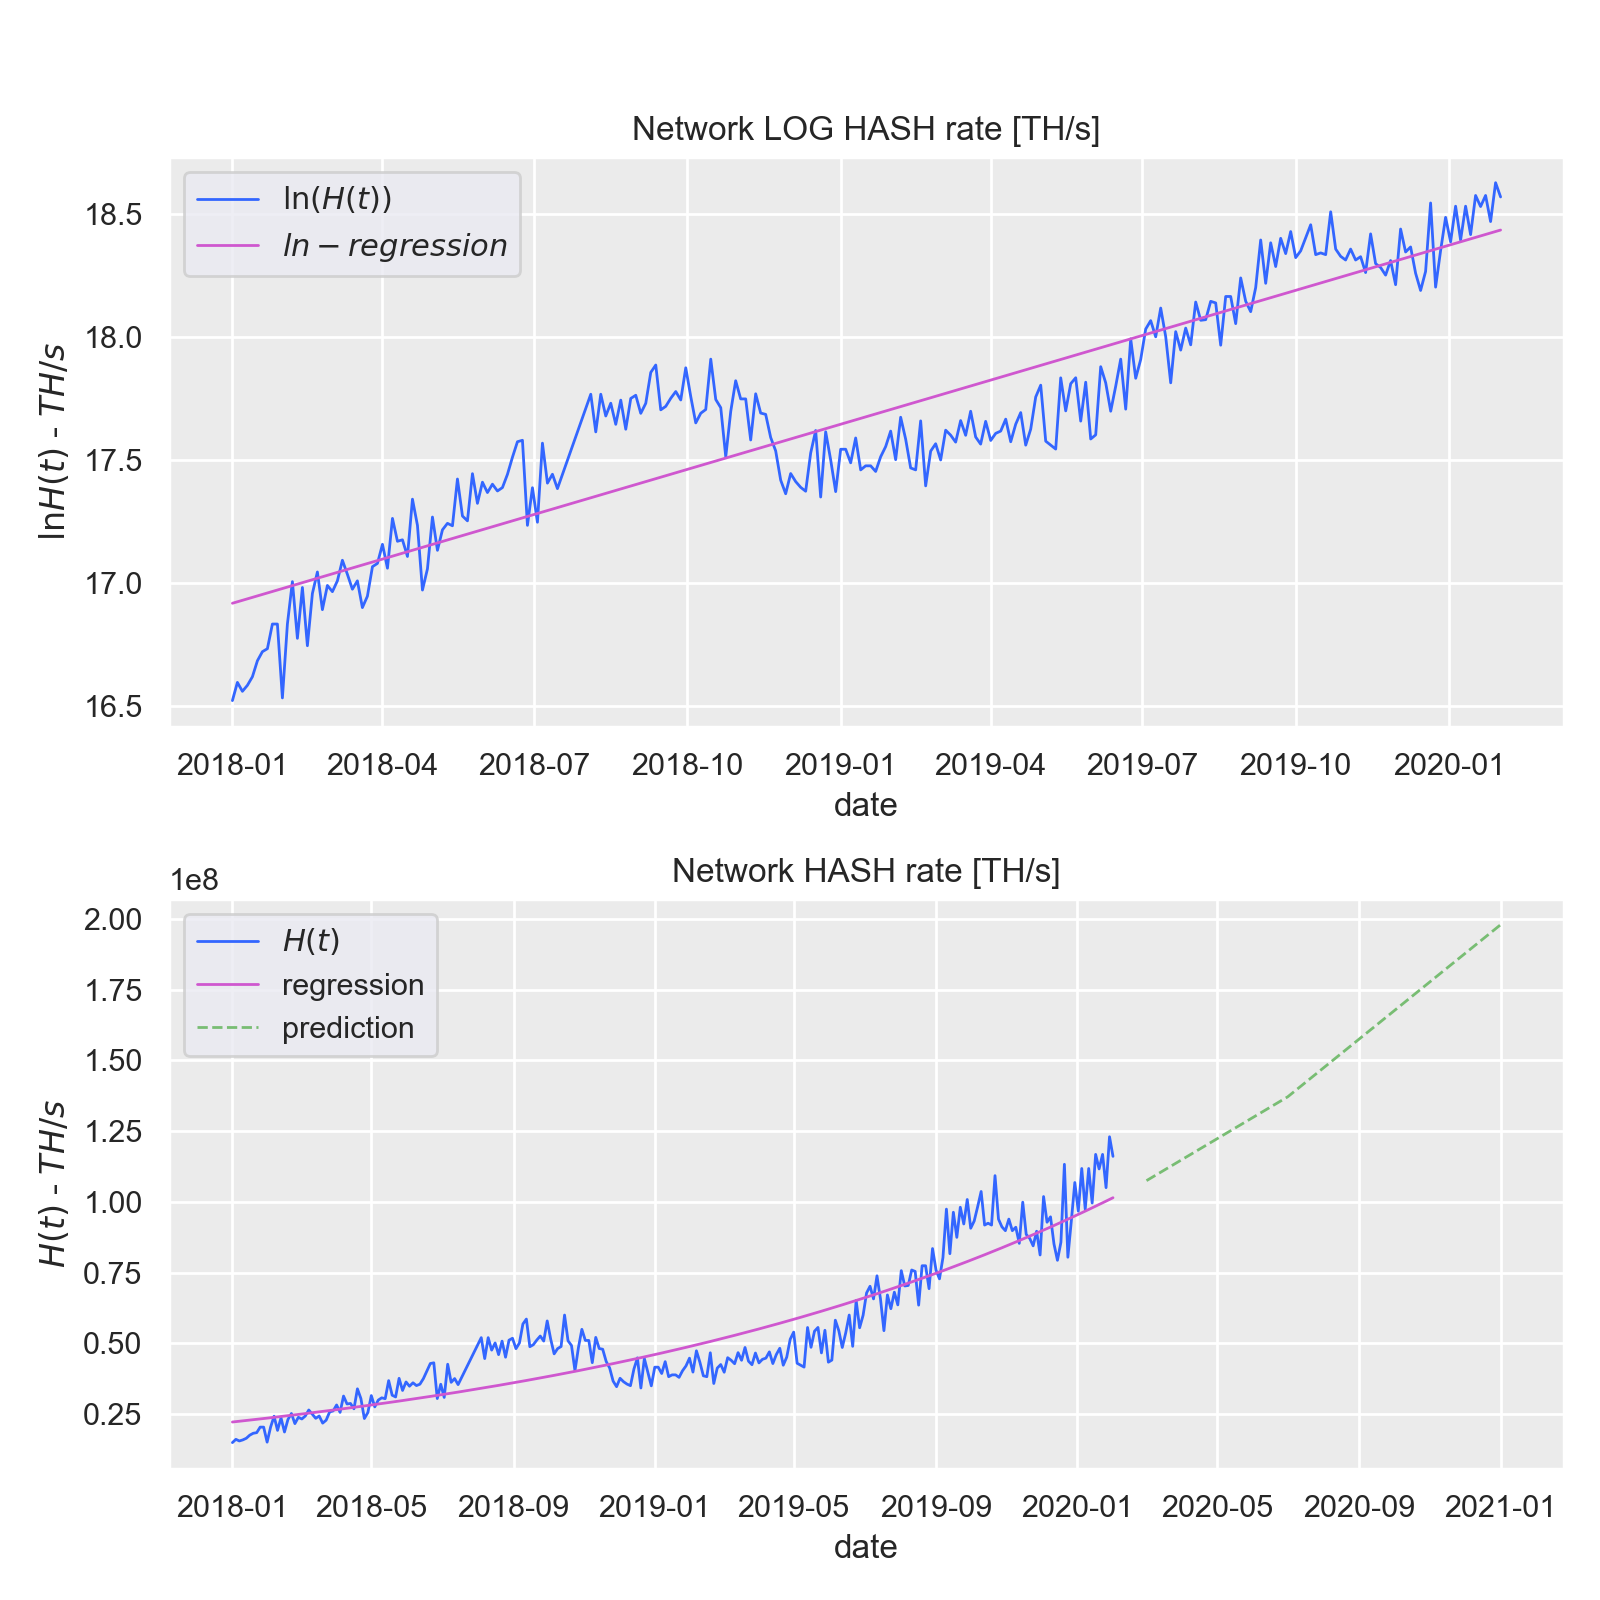
\includegraphics[width=1.0\textwidth]{img/bitcoin-hash-rate.png}
    \caption{Global log-hash rate of the Bitcoin network from Jan, 2018 to Feb, 2020.}
    \label{fig:hash_power}
\end{figure}

The global hash rate can be esteemed indirectly through the difficulty that is recorder in the block header:

\begin{equation}
    \widehat{H_{i}} = \frac{2^{32}}{600} \cdot D_{i+1} \label{H_estimate}
\end{equation}

We have downloaded the estimated network hash rate fome the website \href{https://www.blockchain.com/}{blockchain.com}.

The Figure (\ref{fig:hash_power}) shows the natural logarithm of the hash rate growth $\ln(H(t))$ from Jan 1, 2018 to Feb 1, 2020.

The time unit is seconds ($s$), and the format is the unix epoch, thus seconds elapsed from January 1, 1970.

The hash rate unit is tera hashes per seconds ($TH/S$).

Given the data, we have fit the data to a line using the log-linear regression:

\begin{equation}
    \ln(\widehat{H}(t)) = m \cdot t + q  \label{eq1}
\end{equation}

from which we have derived:

\begin{equation}
    \widehat{H}(t) = e^{q} \cdot e^{m \cdot t} \label{hash_predictor}
\end{equation}

Equation (\ref{hash_predictor}) serves as a \textbf{short term predictor} for future global hash rate values.

The regression exhibits an acceptable fitness to the data. In the future developments of this method, we will show errors and residuals.

We know that growth might rise or decline, but the behaviour is reasonably log-linear since 2014.

Fitting the data, the parameters of the equation (\ref{hash_predictor}) are the following values:

\begin{equation}
    \left \{
        \begin{array}{ll}
            m \approx +2.29 \cdot 10^{-8} \\
            q \approx -17.82
        \end{array}
    \right. \label{values}
\end{equation}

\section{Probability of winning a block}

The Bitcoin protocol is coded to adjust the difficulty in such a way that the expected time to build a block is 10 minutes (600 seconds).

So we can imagine the rent-seeking competition among miners (\cite{theEconomicLimits}) to build a new block as composed of rounds of 10 minutes each.

Given the global network hash rate $H(t)$ and the hash rate owned by a single miner (or mining pool) $h(t)$, we can compute the probability $p_{win}(t)$ of gaining the subside $S_{block}$ for a single round $r(t)$ that starts at $t$ and ends at $t+600$ seconds under the assumption that all the competitors use the "same technology" and the "same algorithms".

The same algorithms assumption seems to be accepted as guaranteed by the Bitcoin protocol and by the nature of the Proof of Work and its cryptographic hash functions (the underlying probability distribution is uniform) that entitles us to consider the random variables independent and identically distributed.

The same technology assumption is weak and serves to overcome some issues related to networking and other minors and majors issues.

The probability is:

\begin{equation}
    p_{win}(t) = \frac{h(t)}{H(t)} \label{eq2}
\end{equation}

In our scenario, $h(t)$ is constant in time and it is much lower than $H(t)$: 

\begin{equation}
    h(t) = h_{o} \ll H(t) \label{eq3}
\end{equation}

So we can write:

\begin{equation}
    p_{win}(t) = \frac{h(t)}{H(t)} = \frac{h_{0}}{H(t)} \label{eq4}
\end{equation}

\section{Expectation}

We can define a random variable $X$ such that:

\begin{equation}
X = \left\{
        \begin{array}{ll}
            X = 1 \textit{, if the miner wins the round} \\
            X = 0 \textit{, if the miner loses the round}
        \end{array}
    \right \} \label{rndX}
\end{equation}

The expected value of X over $n$ rounds is:

\begin{equation}
    \mathbf{E}(X) = \displaystyle\sum_{r=1}^{n} 1 \cdot p_{win}(t(r)) + 0 \cdot ( 1 - p_{win}(t(r))) \label{eq5}
\end{equation}

Where:

\begin{equation}
    t(r) = t_{(r=1)} + 600 \cdot r \label{eq6}
\end{equation}

Rearranging the preceding equations we can write:

\begin{equation}
    \mathbf{E}(X) = \displaystyle\sum_{r=1}^{n} \frac{h0}{\widehat{H}(t(r))} \label{expectationPwinOverRounds}
\end{equation}

Given equation (\ref{expectationPwinOverRounds}) the following code follows:

\begin{lstlisting}[language=Python]
# --------------------------------------------------
# Compute the expected value of X
# --------------------------------------------------

E = 0
r = 0

while(r <= 365 * 24 * 6): # e.g. 1 year
    r += 1
    E += h0 / H(t(r))

return E
\end{lstlisting}

Or, if we want to compute the expected number of rounds needed to win a block:

\begin{lstlisting}[language=Python]
# --------------------------------------------------
# Compute the number of rounds needed to win a round
# --------------------------------------------------

E = 0
r = 0

while(E < 1): # e.g. 1 win
    r += 1
    E += h0 / H(t(r))

return r
\end{lstlisting}

\section{Results}

Given a single high-end commercial ASIC device, the hash rate is $h_{0} = 73\ TH/s$ and under our assumptions
the expected number of wins in a year, starting from Feb. 2, 2020, is:

\begin{equation}
    \mathbf{E}(X) = \displaystyle\sum_{r=0}^{365*24*6} p_{win}(t(r)) \approx 0.026 \label{res1}
\end{equation}

Obviously, given $N=100$ devices of the same model, the result is:

\begin{equation}
    \mathbf{E}(X) = \displaystyle\sum_{r=0}^{365*24*6} p_{win}(t(r)) \approx 2.58 \label{res11}
\end{equation}

\section{Economic prospects drafts}

In this paragraph, we show two simplified economic prospects.

Given the exhibited exponential growth of the global hash-rate, and given the fact that ASIC devices are not repurposable, we have decided to take into account all the device cost without amortization.

Given the BTC price fluctuation (volatility), we have also avoided taking account of interests rates.

\begin{figure}[ht]
    \centering
    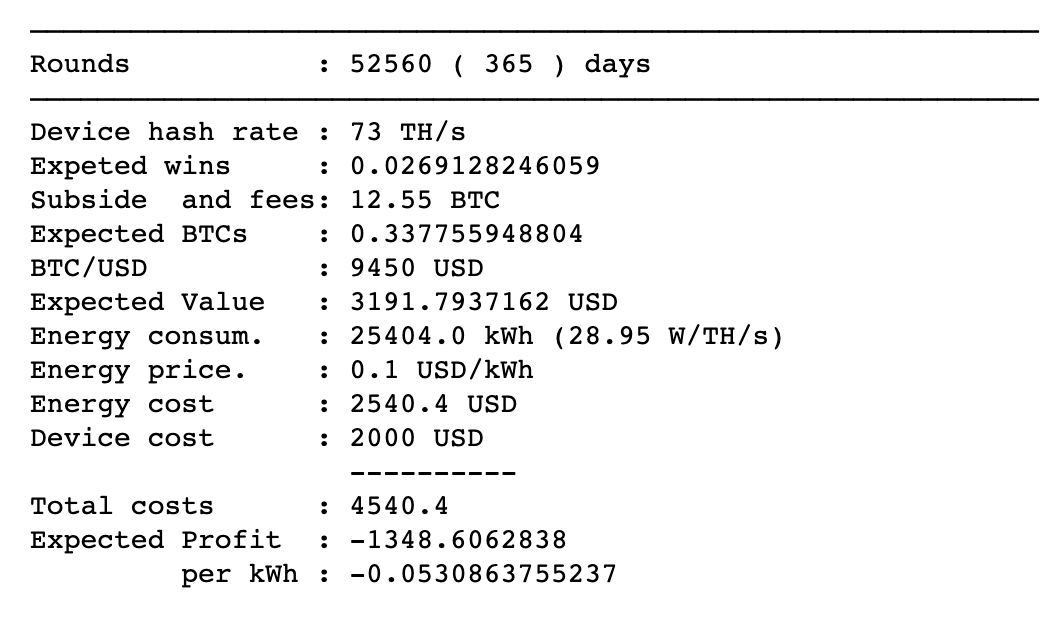
\includegraphics[scale=0.50]{img/results-12.png}
    \caption{Model results for $S = 12.5 BTC$}
    \label{fig:results-12}
\end{figure}

\begin{figure}[ht]
    \centering
    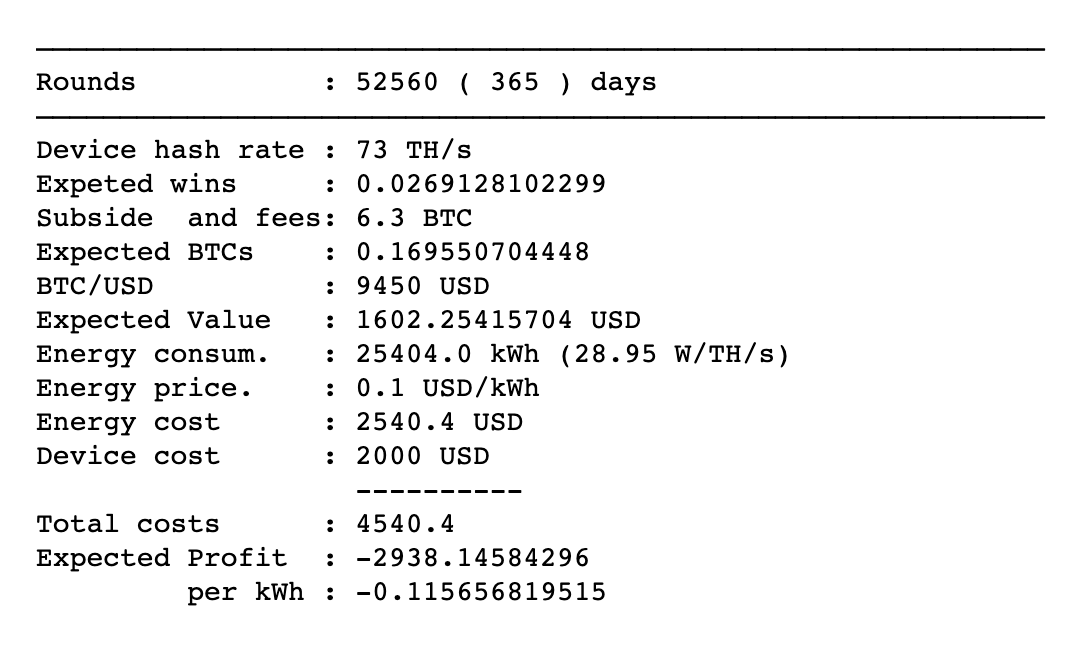
\includegraphics[scale=0.50]{img/results.png}
    \caption{Model results for $S = 6.25 BTC$}
    \label{fig:results}
\end{figure}

\clearpage

\subsection{Simulazione arrivo blocchi}

Di seguito analizzeremo le relazioni che ci contentiranno di costruire un simulatore.
Per simulare un processo futuro non possiamo fare ricorso alla stima sperimentale del valore di $H$, 
ma faremo uso della funzione di crescita esponenziale $\hat{H}$ che ci consentirà di predirre valori futuri a breve termine.


\subsubsection{Processo di Poisson}

Assumendo che l'arrivo di hash validi segua un processo di Poisson (riferimenti), chiamiamo $r$ il numero di eventi nell'unità di tempo:

$$
r = \frac{h}{2^{32} \cdot D}
$$

$\lambda$ è dunque data dalla relazione:

\begin{equation}   
    \lambda = r \cdot t = \frac{h \cdot t}{2^{32} \cdot D}  \label{lambda_rate}
\end{equation}

la densità di probabilità segue la legge:

$$
    \mathbb{P}(\textit{k eventi in t}) = \frac{(r \cdot t)^{k} \cdot e^{-r \cdot t}}{k!}
$$

in particolare per $k = 1$ (1 evento):

\begin{equation}    
    \mathbb{P}(\textit{1 evento in t}) = (r \cdot t) \cdot e^{-r \cdot t}
\end{equation}


il valore medio e la varianza equivalgono a $\lambda$:

$$
    \mathbb{E}(X) = \sigma^{2}(X) = r \cdot t = \lambda
$$

da cui

$$
    \sigma(X) = \sqrt{\lambda} 
$$

Attraverso il metodo proposto da Knuth possiamo generare eventi che seguono la distribuzione:

$$
    \mathbb{P}(T_{1} \le t) = 1 - e^{-r \cdot t}  = \Rightarrow e^{-r \cdot t} = (1 - \mathbb{P}) \Rightarrow t = - \frac{\log_{e}(1 - \mathbb{P})}{r}
$$

\subsubsection{Trattazione dinamica semplificata}

La frequenza di hash globale della rete è dinamica.
Durante il k-esimo round, assumendo i intero positivo tale che $i = \frac{k}{2006}$, per quanto codificato dal protocollo possiamo scrivere:

$$
    \bar{H}_{i} = \frac{2^{32}}{600} \cdot D_{i+1}
$$

sostituendo nella (\ref{lambda_rate}):

$$
\bar{\lambda}_{i} = r_{i} \cdot t = \frac{D_{i+1}}{D_{i}} \cdot \frac{t}{600}
$$

$D_{i+1}$ è calcolato dopo 2016 blocchi per tentare di imporre $\lambda_{i+1} \cdot T_{(i+1)}^{(2016)}  = 2016$ 

Dunque assumendo una legge dinamica per $\bar{H}(t)$, desunta dai valori storici, possiamo ricavare $\lambda$ e simulare il processo degli arrivi.

Vogliamo trovare un valore $\lambda$ che ci consenta di simulare la batteria i-esima. Sappiamo con certezza che nel corso della i-esima batteria $D$ non varia, ma H sì. Duqnue dobbiamo trovare un lambda adeguato a decrivere la densità di probabilità nell'intervallo considerato.

Per semplicità ci riferiremo ad una intera batteria.

Utilizzeremo il predittore $\hat{H}$ ricavato nel paragrafo (\ref{stima_hash_growth}) per simulare una serie di batterie di mining.

Possiamo riformulare la (\ref{hash_predictor}) in questo modo

$$
	\hat{H}(t) = e^{m \cdot t + q} = e^{q} \cdot e^{m \cdot t} = Q \cdot e^{m \cdot t}
$$

Una batteria di round inizia all'istante $t_{0}$ e termina in $t_{0} + T_{2016}$. $T_{2016}$ corrisponde all'istante di arrivo del blocco numero 2016 (di batteria). Per costruzione, $T_{2016}$ approssima $T_{2W}$ che è pari a 2 settimane corrispondenti a $14 \cdot 24 \cdot 60 \cdot 60 = 1,209,600$ secondi. 
Ciononostante, in ragione della dinamicità di $H(t)$, che pur se \textbf{non monotona} tende a crescere, $T_{2016}$ tende ad essere inferiore a $T_{2W}$. Al termine della batteria, il codice re-imposta la difficoltà utilizzando il fattore moltiplicativo:

$$
    k = \frac{T_{2W}}{T_{2016}}
$$

in maniera tale che

$$
    D_{i+1} = k \cdot D_{i}
$$

Dalla quale si ricava il rapporto

$$
    k = \frac{T_{2W}}{T_{2016}} = \frac{D_{i+1}}{D_{i}} = \frac{\bar{H}_{i}}{\bar{H}_{i-1}}
$$ 

dunque

$$
    k = \frac{\hat{H}(t_{0} + T_{2016})}{\hat{H}(t_{0})}
$$

attraverso la quale ricaviamo

$$
\frac{Q \cdot e^{m \cdot (t_{0} + T_{2016})}}{Q \cdot e^{m \cdot (t_{0})}} = \frac{ Q \cdot e^{m \cdot (t_{0})} }{ Q \cdot e^{m \cdot (t_{0})} } \cdot e^{m \cdot T_{2016}} = e^{m \cdot T_{2016}} = \frac{T_{2W}}{T_{2016}} 
$$

$$
    e^{m \cdot T_{2016}} = \frac{T_{2W}}{T_{2016}}
$$

da cui

$$
m = \frac{1}{T_{2016}} \ln(\frac{T_{2W}}{T_{2016}})
$$

riformulando

\begin{equation}
    T_{2016} \cdot e^{m \cdot T_{2016}} - T_{2W} = 0 \label{FuncT2016}
\end{equation}

Se poniamo $T_{2016} = 2016 \cdot T_{mean}$, possiamo trovare una espressione per il tempo medio di mining di un blocco:

$$
    e^{m \cdot 2016 \cdot T_{mean}} = \frac{600}{2016 \cdot T_{mean}}
$$

Per convenienza utilizzeremo il metodo di Newton–Raphson per risolvere numericamente la (\ref{FuncT2016}) precedente, ricavandone un valore approssimativo per $T_{2016}$

\begin{equation}
    f(x) = x \cdot e^{mx} - T_{2W}
\end{equation}

A questo punto, avremo a disposizione $r$ per la batteria in corso:

$$
    \hat{r} = \frac{2016}{T_{2016}}
$$

e questo sarà il valore che utilizzeremo per generare gli eventi del processo di Possion.

Si noti che:

\begin{equation}
    \int_{t_{0}}^{ t_{0} + T_{2016} } \hat{H}(t) \ dt = \bar{H} \cdot T_{2016}
\end{equation}

\subsubsection{Trattazione con processo non omogeneo}

\begin{equation}
    \tilde{\Lambda}(\tau, t) = \int_{0}^{t} r(t) d\tau
\end{equation}

Assumendo

\begin{equation}
    \tilde{\Lambda}(\tau, t) = \int_{t_{0}}^{t_{0} + T_{2016}} r_{0} \ e^{m t} \ d\tau
\end{equation}

\textbf{Integrare}

\newpage

\section{Conclusion}

Many input variables condition the profitability of the mining activity.

For example, the BTC price and fees, the global hash-rate growth, the energy and devices costs, and so on. Further, we should take into account network costs and others.

So, we should refine this method, but it serves as a starting point to debate and improve current public available practices.

This note highlight that within the assumptions and the given costs, solo-mining (or participating in a small pool) is hardly-profitable and poses some questions that we would further investigate:


\begin{itemize}
    \item The cost of electric energy has a high impact on profitability. In which condition we might reduce energy costs?
    \item To take account of other factors that have an impact on the marginal utility (e.g. privacy)
    \item Is the ASIC market overrated? Considering that the devices are not repurposable and the obsolescence rate is very high, the current commercial price seems unjustified.
    \item The system seems to be under the pressure of centralizing forces (both geographically and economically). What will change in the next future? The BTC price? The hash-rate growth? What else? How?
\end{itemize}

With this note, we would give publicity to the fact that the end-user market needs a better model to compute profitability.The proposed method is a point where to start reasoning.

\newpage
\appendix

\newpage
\section{Appunti sul codice bitcoin-core}

\newpage
\section{Glossario}

\newpage
\bibliographystyle{plain}
\bibliography{references}

\end{document}